\documentclass{article}
\usepackage{geometry}
\geometry{letterpaper}
\geometry{margin=1in}
\usepackage{graphicx,graphics}
\usepackage{fancyhdr}
\usepackage{amssymb,amsmath,mathrsfs,amsfonts,amsthm, color}
\usepackage{latexsym}
\usepackage{array}
\usepackage{bm}
%\usepackage{lastpage}
%\usepackage{longtable}
\usepackage{float}
\usepackage{epstopdf}
\usepackage[dvips]{epsfig}
\usepackage{subfigure}
\usepackage{cite}
\usepackage{caption}
\usepackage[backrefs]{amsrefs}
%\usepackage{showkeys}

\pagestyle{fancy}
\fancyhead{} % clear all header fields
\fancyhead[LE]{\thepage}
\fancyhead[RO]{\thepage}
\fancyhead[CE]{\sc G.~Lankford}
\fancyhead[CO]{\sc Universal Identifier}
\fancyfoot{} % clear all footer fields
%\fancyfoot[C]{\thepage}
%\renewcommand{\headrulewidth}{0.0pt}
%\renewcommand{\footrulewidth}{0.0pt}
%\addtolength{\headheight}{2.5pt}

\theoremstyle{plain}			% use "default" font
\newtheorem{thm}{Theorem}[section]
\newtheorem{lemma}[thm]{Lemma}
\newtheorem{prop}[thm]{Proposition}
\newtheorem{cor}[thm]{Corollary}
\newtheorem{conj}[thm]{Conjecture}

\theoremstyle{definition}		% use "definition-style" font for the rest
\newtheorem{defn}[thm]{Definition}

\theoremstyle{remark} 
\newtheorem{rmk}[thm]{Remark}

\newenvironment{acknowledgments}{{\flushleft \bf Acknowledgment:}}{}

\numberwithin{equation}{section}
\numberwithin{figure}{section}
\numberwithin{table}{section}

\renewcommand{\arraystretch}{1.3}
\setlength{\tabcolsep}{2.5mm}
\allowdisplaybreaks[1]





%\title{Gotta Catchem' All: Orbital Space Debris}
%\author{Luis Aguirre, Arezou Ghesmati, Avary Kolasinski, George Lankford,\\
% Scott Spencer, and Stan Swierczek}

\pagebreak

\begin{document}
	
\begin{titlepage}
	\begin{center}
		\vspace*{1cm}
		
		\huge
		\textbf{Universal Identifier:} Who Are You?
		
		
		\vspace{1cm}
		
		\LARGE{Team Target}
		
		\vspace{0.3 cm}
		\large{Niles Armstrong, An Do, Arezou Ghesmati,\\ Alex Happ, George Lankford,
			and Ding Zhao}
		
		\vspace{1cm}
		
		
		%\includegraphics[width=6in]{team_shatterproof_glass_logo.jpg}
		
		\vfill
		
		\begin{flushright}
		\Large
		Proposal for Universally Identifying Users using 
		
		\vspace{0.3cm}
	
		\Large
		Math to Industry Boot Camp (IMA), July 2016
		\end{flushright}
				
	\end{center}
\end{titlepage}
	
%\maketitle
\section{Introduction}
Effective business strategies always involve understanding their customers. A successful business should be cognizant of how their customers use the resources provided for them. While information can be gathered on a more general level, the variability of the demand of individuals can be very high. This is particularly important when trying to give the shoppers that use Target's website a satisfying visit. Thus, by uniquely identifying customers, a more personalized shopping experience can be provided to the customer. The technological age has made the problem of identifying a distinct customer feasible with the amount of data being recorded and stored. Simultaneously, this problem is complex due to people interacting with businesses through multiple channels (store, website, coupon sites, etc.) and through multiple devices (desktop, mobile, phone). This work provides an algorithm that will provide a constrained solution to this problem. In Section 2, the assumptions and methodology for the data to test the algorithm is provided. Section 3 gives the algorithm that will be used to uniquely identify customers from the data. Next, Section 4 will provide data and the results from using the algorithm. Section 5 will discuss the results and provide the pitfalls that will need to be addressed in future research. Finally, Section 6 will give concluding remarks.

\section{Data Generation}
The first step to identifying customers is understanding the data that is available about them. In order to keep the anonymity of customer information, synthetic data needed to be created. The first step was to decide what preliminary assumptions needed to be made about the form and the content of the data.\\
\\
The data that is generated come from records of visits to Target's website. Information gained from store visits are not considered for this work. Customer website visits are be described as one of four scenarios.  A customer will come to the website via a device (desktop, laptop, cellphone or tablet) and
\begin{enumerate}
\item 
look at products with no purchase.  
\item 
purchase an item with a credit card. 
\item 
logs in as a member but makes no purchase.
\item
logs in as a member but makes a purchase with a credit card.
\end{enumerate}
The identifiers that are considered from these scenarios are
\begin{itemize}
\item browser cookies,
\item login username,
\item email address,
\item and credit card number (hashed).
\end{itemize}
An email address being observed from the scenarios is considered a guest email address or combined with its username.  The reasoning is that every username is associated with an email so they are considered the same for simplicity. Table \ref{scenario_tab} shows the information that is gained from each scenario. 
\begin{table}[H]
\centering % used for centering table
\begin{tabular}{| c | c | c | c | c |} % centered columns (8 columns)
\hline %inserts double horizontal lines
Scenario & Cookie & Username & Email & CC\\ [0.4ex] % inserts table
\hline
1 & x & 0 & 0 & 0\\
2 & x & - & - & x\\
3 & x & x & 0 & 0\\
4 & x & x & 0 & x\\
\hline %inserts single line 
\end{tabular}
\caption{The ``x", ``-", and ``0" means this information is, might, or not gained, respectively.} % title of Table
\label{scenario_tab} % is used to refer this table in the text
\end{table}
Many devices and web browsers (Safari, Google Chrome, Firefox, Internet Explorer, etc.) are used to visit the website. Thus, customers can be associated with a multitude of different cookies. For example, an individual could be linked to 2 different cookies where one is from their mobile phone through Safari and the other is using their desktop using the same browser. Another situation is a cookie's lifetime depends on how often a user clears their cookies. If a cookies are cleared often then many cookies can be connected to one person. \\ 
\\
Consider the following simple example to illustrate how the data is generated. A person goes to the website using their laptop, logs in, and purchases items. A few days later, they come back to the site and purchases another product using their desktop as a guest, but uses the same credit card as the first time. This example is represented in figure (a).  A node represents an identifier gathered when the website is visited. An edge indicates that the two nodes were gathered during one visit. The number on the edges is the frequency a link is formed between the 2 nodes. That graph can be described by the table in figure (b) where the number in each cell is the number on a edge that links two nodes. Figure (c) is the adjacency matrix formed from figure (a) and figure (b).  
\begin{figure}[H]
\centering 
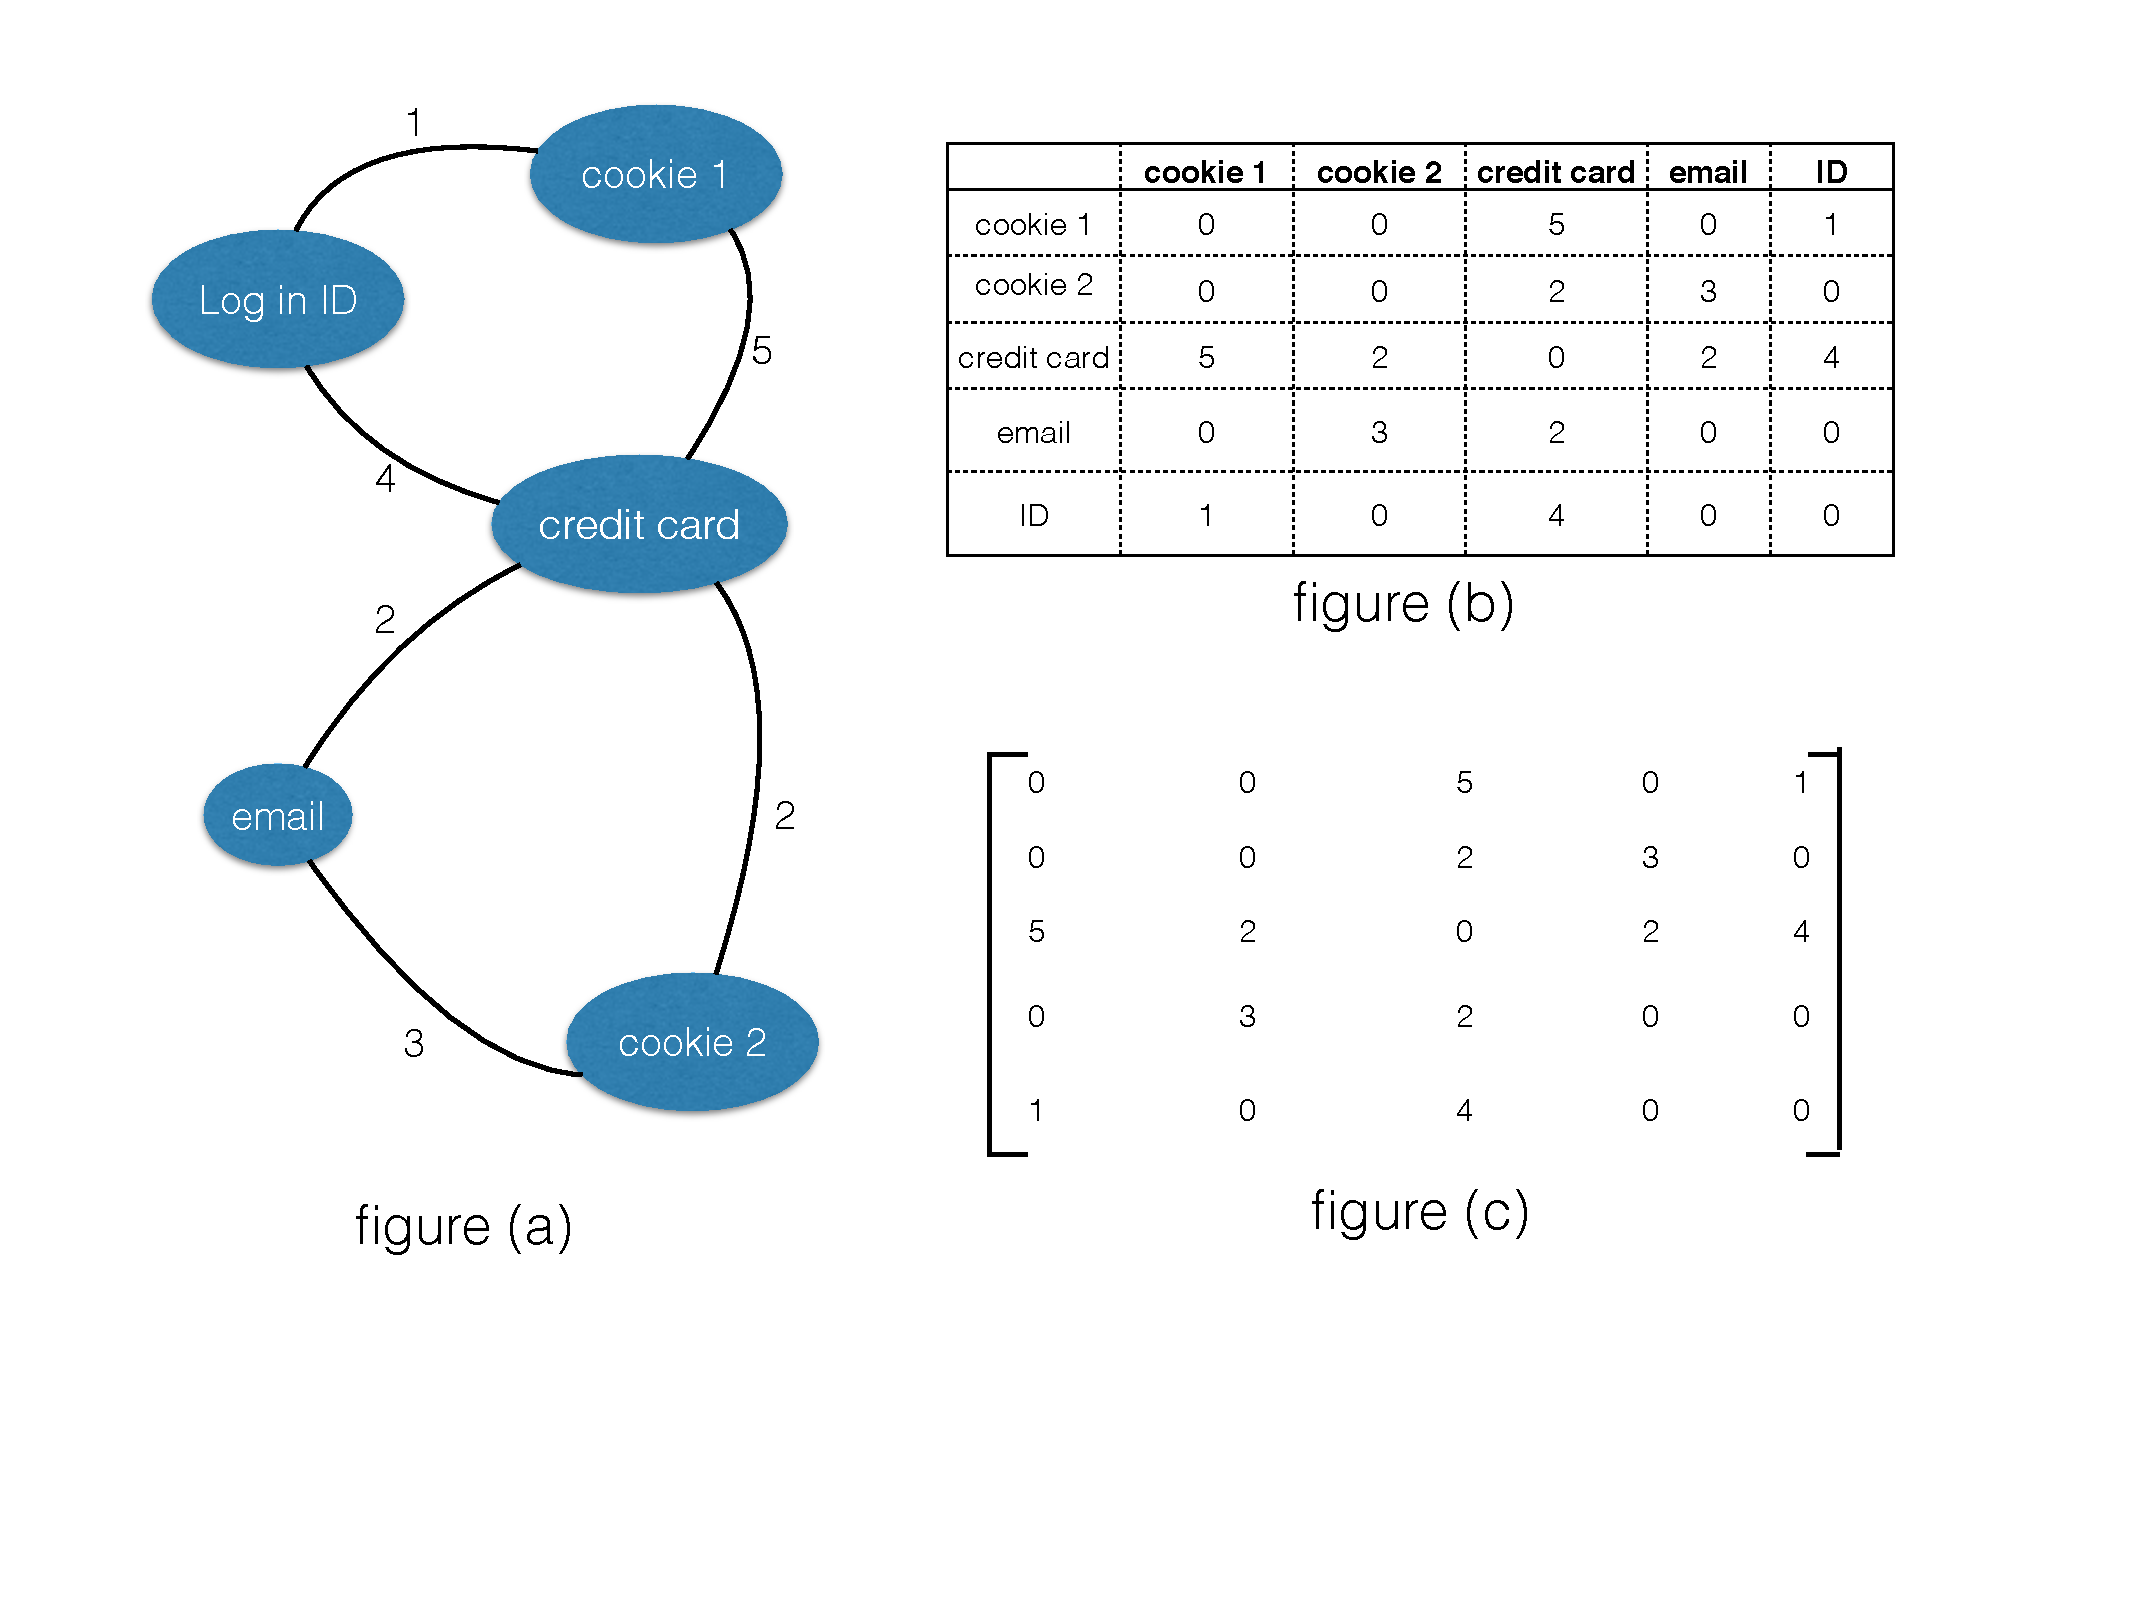
\includegraphics[scale=.3]{graph}
\end{figure}
The example above is for one person. The data that is generated can be for multiple people as well. The number of identifiers is randomized as well as the number of times each one is linked. The graphs that are generated are k-partite graphs. Thus, no two identifiers of the same kind can have an edge between them. Then, an adjacency matrix is made using this information. This adjacency matrix is used in the algorithm developed in the next section.



\section{Algorithm}
\section{Complexities and Future Research}
Scenario 1 is considered a \textit{dangling cookie} and is not very useful in this context because it gives no link to a particular user. 

Over the last three decades, orbital debris has progressed from a nearly unknown problem to a recognized issue being addressed at the international level. There are many organizations in the United States and around the world that are involved in guidelines and policies for space debris prevention. In 1981, the Department of Defense (DOD) observed that second stage explosions made a considerable amount of debris. In order to eliminate future explosions, they decided to deplete and vent excess fuel and oxidizer. In 1995, NASA was the first organization in the world to give a set of formal guidelines specifically for orbital debris mitigation. The U.S. Air Force's Space and Missile Systems Center (SMC) decided to put hard requirements on contracts for new system designs to optimize space debris prevention. There are more options for designs that are easier and less expensive if debris mitigation alternatives are considered earlier. The Aerospace Corporation published the SMC Space Debris Handbook in 2002 to ensure that space debris reduction requirements are considered into system designs. Federal Aviation Administration (FAA) certification requires that an applicant demonstrate that the risk level associated with the debris from a proposed launch meets the public risk criteria for unplanned explosions. The Federal Communications Commission (FCC) developed orbital debris mitigation rules focused on communications satellites in Earth orbit. For example, an end-of-life plan (EOLP) is required that details the post-mission disposal strategy. This includes the quantity of fuel that will be reserved to perform post-mission disposal maneuvers. For GEO orbit satellites, the EOLP must disclose the altitude selected for a post-mission disposal orbit.\\
   
The prevention guidelines will help reduce the introduction of new potential debris, but the population of debris is still growing. Collisions generate more space debris which increases the probability of future collisions.  As noted earlier, this could be catastrophic for the over \$150 billion ISS. Therefore, research and development debris mitigation methods are important steps to preserve space for future generations. The next section will give a brief description of potential methods and the method that will give the most optimal cost and efficiency for extraction of debris.
%"Disaster is not immidiate, but the
%need for mitigation action is now.
%Real money must be spent on
%real programs now to benefit a
%somewhat vague future. "

\section{Mitigation Methods}
There are many different proposed strategies for removing orbital debris that include balloons, aerogel catcher's mitt, satellites with arms, lasers, and satellites with nets.  The balloons push any debris into the atmosphere, but do not work efficiently in the higher altitudes of the LEO which is where a good portion of the pieces are located.  The aerogel catcher's mitt captures debris of all sizes, however, it is estimated to cost about a trillion dollars just to launch which is unreasonable.  The satellites with arms are a feasible option that grab and destroy larger pieces of debris, but many satellites would be needed to make a significant impact since they self-destruct with the pieces.  Thus, after extensive research, the lasers and satellites with nets were observed to be the most promising. This section will provide a comparison for these two methods.  The lasers will be the first option that is considered.
\subsection{Lasers}
Laser Orbital Debris Removal (LODR) is a ground-based mitigation option. A large mirror or array of mirrors, ideally 13$+$ meters in diameter, would be used to focus on the debris as it passes across the sky. Given the average radial velocity of debris in LEO, there would be a window of approximately 100 seconds to focus the mirror on the leading edge(s) of the object. The laser vaporizes some small portion of the object's surface, and causes a small adjustment to its orbital path. For objects with mass less than 10 kg, a single pass will alter the objects orbital path causing it to burn up in the upper atmosphere. For larger objects with mass over 1,000 kg, multiple passes are required, and the process may take years for the object's orbit to be altered enough to obtain the desired effect. However, because of the short pass time, several different objects can make a pass each day. This allows most of the objects with diameter 100 cm or greater to be removed within about a five year period.\\
\\
One disadvantage is that the LODR requires a large investment. Currently, there are no finished mirrors of the required size, although there are several under construction. The largest completed telescope mirror has a diameter of about 10 meters, and cost \$200 million to construct with annual operating costs of \$20-30 million. There are additional requirements that would likely increase the construction costs to roughly \$1 million for each large object that is removed, and \$5,000-10,000 for each smaller object. These costs among other attributes, make the satellites with nets a more attractive option.
\subsection{Satellites with Nets}
In the interest of price and feasibility, there has been an enticing proposal in using satellites with nets.  There are two main nets that have been developed thus far: the Japan Aerospace Exploration Agency (JAXA) design and the ElectroDynamic Debris Eliminator (EDDE). The JAXA design is powered by solar panels and the Earth's electromagnetic field. A thick tether attaches a large magnetic net that is used to capture any size debris. The JAXA design is one of the cheaper methods and has a long lifespan, but self-destructs similar to the satellite with arms. The EDDE is a more appealing alternative. Star Technology and Research, Inc. introduced the EDDE in 2002 and in more detail in 2009 at the NASA/DARPA conference on orbital debris removal.\\
\\
The EDDE's intricate design allows for substantial total reduction of debris with minimal cost.  Each spacecraft consists of three solar arrays, two electron emitters, and two net managers all connected via a sturdy conductive tape. The solar arrays are used in conjunction with the sun and the Earth's electromagnetic field to generate power. Additionally, they are the brains behind maneuvering the spacecraft through the orbit to catch debris and avoid collisions.  The electron emitters are the main locations that attracts electrons used in acceleration of the spacecraft.  The net managers deploy a retractable net to capture large debris and transport it to a lower orbit to be extinguished by the atmosphere. Then, the net managers reel in the empty net and the EDDE returns to higher orbits for more debris. The EDDE can also collect operating and non-operating satellites to transport to the ISS for repair and/or to dissemble and reuse non-operating satellite pieces. Thus, the EDDE can serve multiple purposes. If damaged and the tether breaks, each end can still function independently. A disadvantage of the EDDE is that it does not remove the small debris. However, it does nearly maximize the total removal and significantly reduces the probability of collisions.\\
\\
Scientists have estimated that launching 16 EDDEs will lead to the removal of 2,000 tons of large debris in approximately 9 years. This reduces the collision of shrapnel production in LEO by over 97\%.  If only 10 EDDEs are launched, a total of 1,000 tons of debris in 7 years will be removed with over 79\% decrease of shrapnel collisions.  The total price for launching and managing 12 EDDE would run about \$84 million per year over 12 years. Table 3.1 gives a detailed breakdown of the cost to remove all large debris using lasers compared to the EDDE. Its multipurpose attributes and low cost make the EDDE the most efficient way to decrease debris in the LEO. In the next section, the EDDE's production is modeled using a time dependent stochastic process.
\begin{table}[H]
\centering
\begin{tabular}{| c | c  | c | }
\hline
Mitigation Method & The EDDE & The ground laser \\
\hline
Total years to remove & 12 & 14 \\
\hline
Total cost to remove all large debris & \$1 billion & \$2.2 billion \\
\hline
\end{tabular}
\caption*{\small{\textbf{Table 3.1}: The cost of the EDDE operation compared to the cost of the ground laser to remove all large debris.  The EDDE operation assumes 12 EDDE's used with \$84 million per year of cost. The ground laser assumes \$1 million to take down one large piece of debris.}}
\label{EDDEtab1}
\end{table}

\section{Proposed Model}
The proposed model describes population growth of objects in LEO as an interactive Markov process with different mean wait times. There are several processes considered that occur concurrently that include:
\begin{enumerate}
\item An average of 120 new satellites are launched on a anual basis.
\item  When a satellite completes its missions, it either returns to the upper atmosphere or becomes large debris. Prevention policy adherence will determine the proportion of satellites that become debris.
\item Depending on the altitude above Earth, debris may eventually decay out of LEO into the atmosphere.
\item Collisions between small debris and nonoperational/operational satellites creates more small pieces of debris. The mean time between
one of these interactions is approximately three years.
\item We may remove large debris using the EDDE.
\end{enumerate}
\vspace{0.3cm}
The focus of this work is to clear the debris in the atmospheric layers around the ISS. There are several layers of LEO that have different densities of
debris and operational satellites. Each layer is modeled separately. The layer corresponding to 800 - 1000 km altitude has the highest debris density, but does not have many operational satellites. The decay from this altitude to lower layers usually takes around a century. The layers from 300 - 600 km (where the ISS inhabits) and 600 - 800 km are of more interest to us because the decay rates to lower orbits are around a year and decade, respectively. Recent data on the overall debris density at each layer and the number of operational satellites in each layer is used for this work. \\
\\
The model includes several event-dependent parameters. The collision probabilities increase when the amount of small debris is higher. If the number of satellites becomes proportionally larger than the initial amount, then the launch rate decreases. If the number of satellites becomes smaller than the initial amount, then the launch rate increases. The rate debris is removed by the EDDE is dependent on how many large pieces of debris are left in the layer. The rate assumes that it takes longer for the EDDE to rendezvous with large debris as quantities decrease. A time dependent rate for when policy constrained satellites are instructed into the Earth's atmosphere upon completion of their service lives is also included in simulations. \\
\\
Simulations are run for a specified number of events. When an operational satellite is struck, a corresponding cost to replace the satellite is appended. The cost breakdown based on the size of the satellite is given by Table 4.1.
\begin{table}[H]
\centering
\begin{tabular}{| c | c  | }
\hline
Size of Satellite & Cost of Collision \\
\hline
Small ($\approx$ 5 kg) & \$50,000 \\
\hline
Medium ($\approx$ 700 kg) & \$100 mil \\
\hline
Large ($\approx$ 2000 kg) & \$400 mil \\
\hline
\end{tabular}
\caption*{\small{\textbf{Table 4.1}: Costs are acquired from averages to replace a satellite.}}
\label{Modeltab1}
\end{table}
After a given number of events occur, the number of wait times, total time (years), and the associated cost in lost satellites are obtained and recorded. The simulation is run several dozen times and the results are averages. This is repeated under four different scenarios:
\begin{enumerate}
\item No prevention policy is implemented and the EDDE is not used.
\item A prevention policy is utilized.
\item The EDDE is employed.
\item A prevention policy and EDDE are both used.
\end{enumerate}

The prevention policy that is applied is that the satellite designs that are built have end of mission disposal plans. As stated earlier, there are implemented guidelines that are not always followed.  In the model, it starts at 50\% adherence and if the prevention policy is implemented, then the adherence increased to 95\% in ten years.
After running all four scenarios, the average cost outputs indicate that the cost of scenario one over 30 years is around \$6 billion in lost satellites. Scenario two gives minimal improvement with mean savings of \$3.5 billion. The cost in lost satellites over 30 years with a 12 year EDDE debris removal program and continued maintenance program has mean of \$1 billion, providing savings to government and industry of \$5 billion.  This cost analysis is consistent with the debris population growth in the different scenarios.  The following table and charts summarize our findings.

%\vspace{2cm}
\begin{table}[H]
\centering
\begin{tabular}{| c | c  | c | c | c|  }
\hline
 Scenario & 1 & 2 & 3 & 4\\
\hline
Cost from Lost Satellites (in billions USD)& 6.16 & 5.56 & 2.51 & 2.56 \\
\hline
Large Debris & 2846 & 2312 & 31 & 11 \\
\hline
Small Debris (x1000) & 104 & 99 & 79 & 79 \\
\hline
\end{tabular}
\caption*{\small{\textbf{Table 4.2}: Costs are acquired from averages to replace a satellite.}}
\label{Modeltab1}
\end{table}

\section{Conclusion}
This proposal finds that the EDDE is the best option for orbital debris removal. This work provides a detailed description and model for implementation of the EDDE and the benefits over other considered methods. This situation is high priority due to the catastrophic losses scientifically and monetarily if the ISS is damaged or destroyed.  We urge the UN to act quickly.




\newpage
\section{Technical Appendix}
\subsection{Details about EDDE}

The ElectroDynamic Debris Eliminator, otherwise known as the EDDE, is the leading contender for removal of large debris from the LEO. The International Astronautical Federation published an extensive paper on the EDDE written by Star Technology and Research, Inc. in 2014. This paper reports the fine details of the makeup and performance of this spacecraft.\\
\\
The EDDE is a space vehicle made up of two net managers, two emitters, and three solar arrays all connected by a sturdy conductive tape. It sails through the ionosphere using power generated by the solar arrays.  Each component of the EDDE is carefully designed to maximize efficiency and decrease overall cost and mass.  Details of each component are described below.
\textbf{Solar arrays}: The main concerns for satellites include the total cost, ongoing maintenance, overall mass, and the total life expectancy.  All of these concerns are directly related to the type of chemical propellant used to power the spacecraft. Many studies have been done comparing different fuels however, the maintenance, cost, lifespan, and mass of the satellite are still significantly affected by even the best fuel. Recently, scientists have overcome these concerns with the EDDE by using solar arrays as generators for power.  EDDE can use as much power as needed while keeping the mass and the cost at a minimum.\\
\\
There are three flexible and lightweight solar arrays evenly distributed at about 400m apart along the length of the conducting tape. Each segment has power and control of electron collection, conduction, and emission, and each end can control overall maneuvers.  This allows for precise regulation of the current and hence control of rotation, rate, and bending dynamics of the spacecraft.  Additionally, since each segment is independent in this way, control is maintained after component failures. For instance, in the case that the conductive tape is cut by a meteoroid or debris, each piece can still thrust and control itself, and can either continue a mission more slowly, or deorbit itself promptly, to prevent danger to other spacecraft that could arise after another tape severance.\\
\\
The solar array has undergone recent modifications concerning the cell type and array design. After many tests, scientists concluded that the best cell type is a bifacial silicon terrestrial-type cell; the main reason being their low cost, low mass, and robustness. The best array design has concluded to be laminating the bifacial cells between layers with clear plastic film.  With these implementations, the array mass has decreased to only about 5 kg/kW. Not only do these features make the solar array lighter and cheaper, but it also appears that it produces more usable power from the same total mass as before.\\
\\
\textbf{Conductive Tape}: Each component of the EDDEE is connected via a sturdy conductive tape. The conductive tape design is one of the most important updated features of the EDDE. It uses a ribbon of aluminum foil 1-3 cm wide that is reinforced with a unidirectional fiber composite layer for strength and tear resistance.  This composite layer greatly reduces vulnerability to small micrometeoroids and debris, which is a large cause in destruction to other satellites in the LEO.  Reinforced foil tapes are much better for the electron collection compared to wires. This is because the tapes have more usable electron collection areas and hence, a wider tape is not necessarily needed to collect more electrons for current. This recent modification to the conductive tape has allowed for a 25\% narrow tape without increasing the risk of tape cut by hypervelocity impacts or decreasing efficency.\\
\\
\textbf{Electron Emitters}: The light solar arrays have lead to an alternative to hollow cathodes as the design for electron emissions.  The analysis of recent data has determined that thermionic electron emitters are both lightweight and efficient. EDDE uses multiple emitters that each emit about 20mA. The plasma anodes in high plasma densities are close enough to each wire that they do not overlap. However, at lower densities, they do.  This increases the space charge bias voltage needed for any give current. This could be a problem but since at low plasma densities the electron collection along EDDE?s tape also drops, the current capability does not reduce as much as collection does hence avoiding the possible problem.\\
\\
\textbf{Net managers}: The EDDE is also equipped with two net managers located at each end.  The net managers deploy large, lightweight nets used to capture objects, and/or satellites and deliver each to its desired orbit.\\
\\
The intricate design of the EDDE allows for fluid and efficient maneuvering through space.  However, since the EDDE is powered by the sun and the Earth's electromagnetic field, EDDE has batteries to ensure that the avionics and communications run at night but does not thrust. That is, EDDE maneuvers in the sun and coasts at night while maintaining the ability to avoid objects. EDDE uses electric current in the conductive tape that reacts against the Earth?s magnetic field. The spacecraft collects electrons from the ambient ionospheric plasma near one end of the tape and ejects them back into the plasma near the other end, using hot-wire electron emitters. The thrust comes from the current in the tape crossing geomagnetic field lines. Average thrust when the EDDE descends is typically much higher than when it climbs, which is extremely advantageous for when EDDE drags down large debris into the lower orbits. This electric current movement has proven to be successful by NASA JSC in 1993 and by NASA MSFC?s TSS-1R in 1996.\\
\\
A key in the fluid movement of EDDE is its rotation, which is controlled by its solar arrays. The spacecraft is deployed already spinning slowly which can stabilize the solar array facing the sun for power as well as provide enough tension to drive EDDE to component release.  After all necessary phases are completed, the spin and tension are increased. This is to improve stability by stiffening the tether against the transverse thrust forces and allows for wider range of angles with geomagnetic field and hence thrust directions. Because of this, EDDE can handle currents and thrusts much higher than previous designs and increases its agility. Additionally, rotation is particularly useful in near-polar orbit for altitude changes, which is the most time consuming part of removing large debris from outer orbits. Performance in these near-polar orbits is critical for debris removal, since over 60\% of the 2,200 tons of LEO mass is within 10 degrees of the polar orbit. This design and rotation sets EDDE apart from previous electrodynamic thruster concepts for LEO. \\
\\
The capturing of large, uncooperative debris is an extremely difficult task. Once a target is detected, EDDE performs free-return successive trajectories to approach the debris. The debris is easy to find when within 100 km due to the bright reflection of sunlight and slow movement across the starfield. The main guidance tool are the cameras located at each end of the EDDE.  The cameras use binocular viewing of the target against the starfield. The free-return trajectory relative to the target reduces the residual error by successive approximation. Two important factors to note are that binocular ranging is only possible when the debris is sunlit, and it is significantly simpler if the background of the debris is a starfield rather than a sunlit Earth. This is easily taken care of with the skilled agility and image processing of the cameras.  As EDDE makes it way to the target debris, the sunlit glare will wash out the starfield backdrop. However, once this occurs, the cameras looking in the other direction provide an adequate view and point reference to keep EDDE along the path to its target.\\
\\
An iterative successive approximation approach strategy allows multiple sunlit inspection passes. This can help verify the tumble rate of the target and ensure that the debris has no unexpected features that would complicate the capture. The actual capture of the debris needs to be extremely accurate thus calling for iterative estimates of the error throughout small time intervals upon the approach.  To capture the large debris, a net manager expends its Spectra net and support lines and the EDDE arranges the target to pass between two net support lines. As the target passes over the center of the net, the net manager quickly retracts the lines to pull the net up around the target. If the cameras suggest problems during the final approach to the target, there are two options for late abort: retract the net early, or don?t retract at all and let the target escape. In addition to uncooperative targets such as debris, EDDE captures cooperative targets as well.  The capturing occurs in the same way as capturing an uncooperative target however, once the target is capture, the EDDE delivers it to a repair facility. After repair, EDDE can pick up and return the cooperative target to its operational orbit.\\ 
\\
It has been estimated that all pieces of large debris in LEO can be completely removed in 12 years by sending up 12 EDDE?s. In this case, the cost per year is estimated to be about \$84 million. Table 3.1 shows the details of this per year budget. Using this approach, it would require about \$1 billion over 12 years to completely clean up the large debris and significantly reduce the LEO debris problem at hand.




\begin{table}[H]
\centering
\begin{tabular}{| c | c  |}
\hline
Description  & Cost\\
\hline
Construction Materials (\$4.5 mil/EDDE) & \$54 mil\\
\hline
Launch Materials (\$5,000-6,000/EDDE) & \$6 mil\\
\hline
Operating Cost (160 satellite/aerospace engineers $\times$ \$150,000 average salary) & \$24 mil\\
\hline
Total  & \$84 mil/year \\
\hline
\end{tabular}
\caption*{\small{\textbf{Table 3.1}: Cost per year for 12 EDDEs.}}
\label{tab_fits}
\end{table}
\subsection{Details about Model}
The rate $\lambda_i$ represents the inverse of the mean wait time between each event per process. The state of the system is an ordered triple $\{S,C,B\}$ where
$$ S = \textnormal{number of operational satellites in current level} $$
$$ C = \textnormal{number of large debris in current level} $$
$$ B = \textnormal{number of small debris in current level} $$
Then the mean wait time between state changes is distributed exponentially with parameter 
$$
\lambda = \sum_{i = 1}^9 \lambda_i.
$$ 
The probabilities of specific state changes are
given by
$$ P_{S+1,C,B}  = \dfrac{\lambda_i}{\lambda}$$
The model begins by generating two random numbers, $r_1,r_2\in (0,1)$, from a uniform distribution on [0,1]. Let the time between events be given by $t$ where
$$t=\dfrac{-\log(r_1)}{\lambda}$$
We use the ratio of probabilities to create bins in this interval and select what event occurred based on $r_2$, the second random number. Depending on which event occurs, there may be an additional random process. Satellites and larger pieces of debris follow a trimodal distribution. A plurality of satellites are only 1 to 5 kg in mass, then there exists a portion of satellites roughly 700 kg in mass, and then a lesser amount of very large satellites with mass around 2000 kg. If our random number falls in the bin for a satellite being struck and broken up, a second random number is generated and based on its
location, a satellite corresponding to the different sizes is broken into a corresponding amount of debris. For example, a small satellite may only generate 10 to 25 pieces of small debris, while a medium satellite may generate 1000 pieces of small debris. \\








%-------------------------References----------------------------%

\begin{bibdiv}

\begin{biblist}



\bib{}{article}{
	AUTHOR = {S. Cardoni},
	TITLE = {5 Ways to Clean Up Space Junk: What Goes Up Should Come Down},
	YEAR = {2011},
	URL = {http://www.takepart.com/article/2011/06/28/5-ways-clean-space-junk},
}


\bib{}{article}{
    AUTHOR = {L. David},
     TITLE = {How to Clean Up Space Junk: DARPA's Orbital Catcher's Mitt},
   %JOURNAL = {IEEE Trans. Inform. Theory},
  %FJOURNAL = {Institute of Electrical and Electronics Engineers},
    %VOLUME = {59},
      YEAR = {2011},
    %NUMBER = {4},
     %PAGES = {2082--2102},
      %ISSN = {0018-9448},
     %CODEN = {IETTAW},
   %MRCLASS = {94A12},
 % MRNUMBER = {3043783},
       URL = {http://www.space.com/11657-space-junk-orbital-debris-cleanup-darpa.html},
}


\bib{}{article}{
	AUTHOR = {J. Heimbuch},
	TITLE = {Giant GOLD Balloon to Clean Up Space Junk},
	YEAR = {2010},
	URL = {http://www.treehugger.com/clean-technology/giant-gold-balloon-to-clean-up-space-junk.html},
}

\bib{}{article}{
	AUTHOR = {J. Perason {,} J. Carroll {,} E. Levin},
	TITLE = {EDDE Spacecraft Development for Active LEO Debris Removal},
	YEAR = {2014},
	URL = {http://www.star-tech-inc.com/papers/EDDE_Debris_Paper_IAC14A664x23806_2014Sept28.pdf},
}


\bib{binarystable}{article}{
    AUTHOR = {C.R. Phipps{,} et. all},
     TITLE = {A Laser Optical System to Remove Low Earth Orbit Space Debris},
   %JOURNAL = {IEEE Trans. Inform. Theory},
  %FJOURNAL = {Institute of Electrical and Electronics Engineers},
    %VOLUME = {59},
      YEAR = {2013},
    %NUMBER = {4},
     %PAGES = {2082--2102},
      %ISSN = {0018-9448},
     %CODEN = {IETTAW},
   %MRCLASS = {94A12},
 % MRNUMBER = {3043783},
       URL = {https://e-reports-ext.llnl.gov/pdf/754322.pdf},
}


\bib{}{article}{
	AUTHOR = {M. Wall},
	TITLE = {Want to Get Rid of Space Junk? Catch It in a Giant Net},
	YEAR = {2011},
	URL = {http://www.space.com/12819-space-junk-cleanup-giant-net-tether.html},
}




\bib{}{article}{
	AUTHOR = { },
	TITLE = { },
	YEAR = { },
	URL = { },
}

\bib{}{article}{
	AUTHOR = { },
	TITLE = { },
	YEAR = { },
	URL = { },
}

\end{biblist}
\end{bibdiv}  


\end{document}